%
% Sección de resultados y conclusiones,
% presentación en RCI.
% Proyecto Lovelace.
%

\section{Resultados y conclusiones}

\begin{frame}{Resultados}
  Las pruebas de desempeño de llevaron a cabo en una computadora con las
  siguientes características:
  \begin{itemize}
    \item \textbf{Procesador:} Intel i5-7200U (2.5 GHz) de 4 núcleos.
    \item \textbf{Sistema operativo:} Arch Linux, kernel 4.18.
    \item \textbf{Base de datos:} MariaDB 10.1.
    \item \textbf{Compilador:} GCC 8.1.1.
  \end{itemize}
  El procesador utiliza los conjuntos de instrucciones de Intel
  AES-NI y RD-SEED~\cite{aesni_wp}.
\end{frame}

\begin{frame}{Resultados}
  \begin{figure}[H]
    \centering
    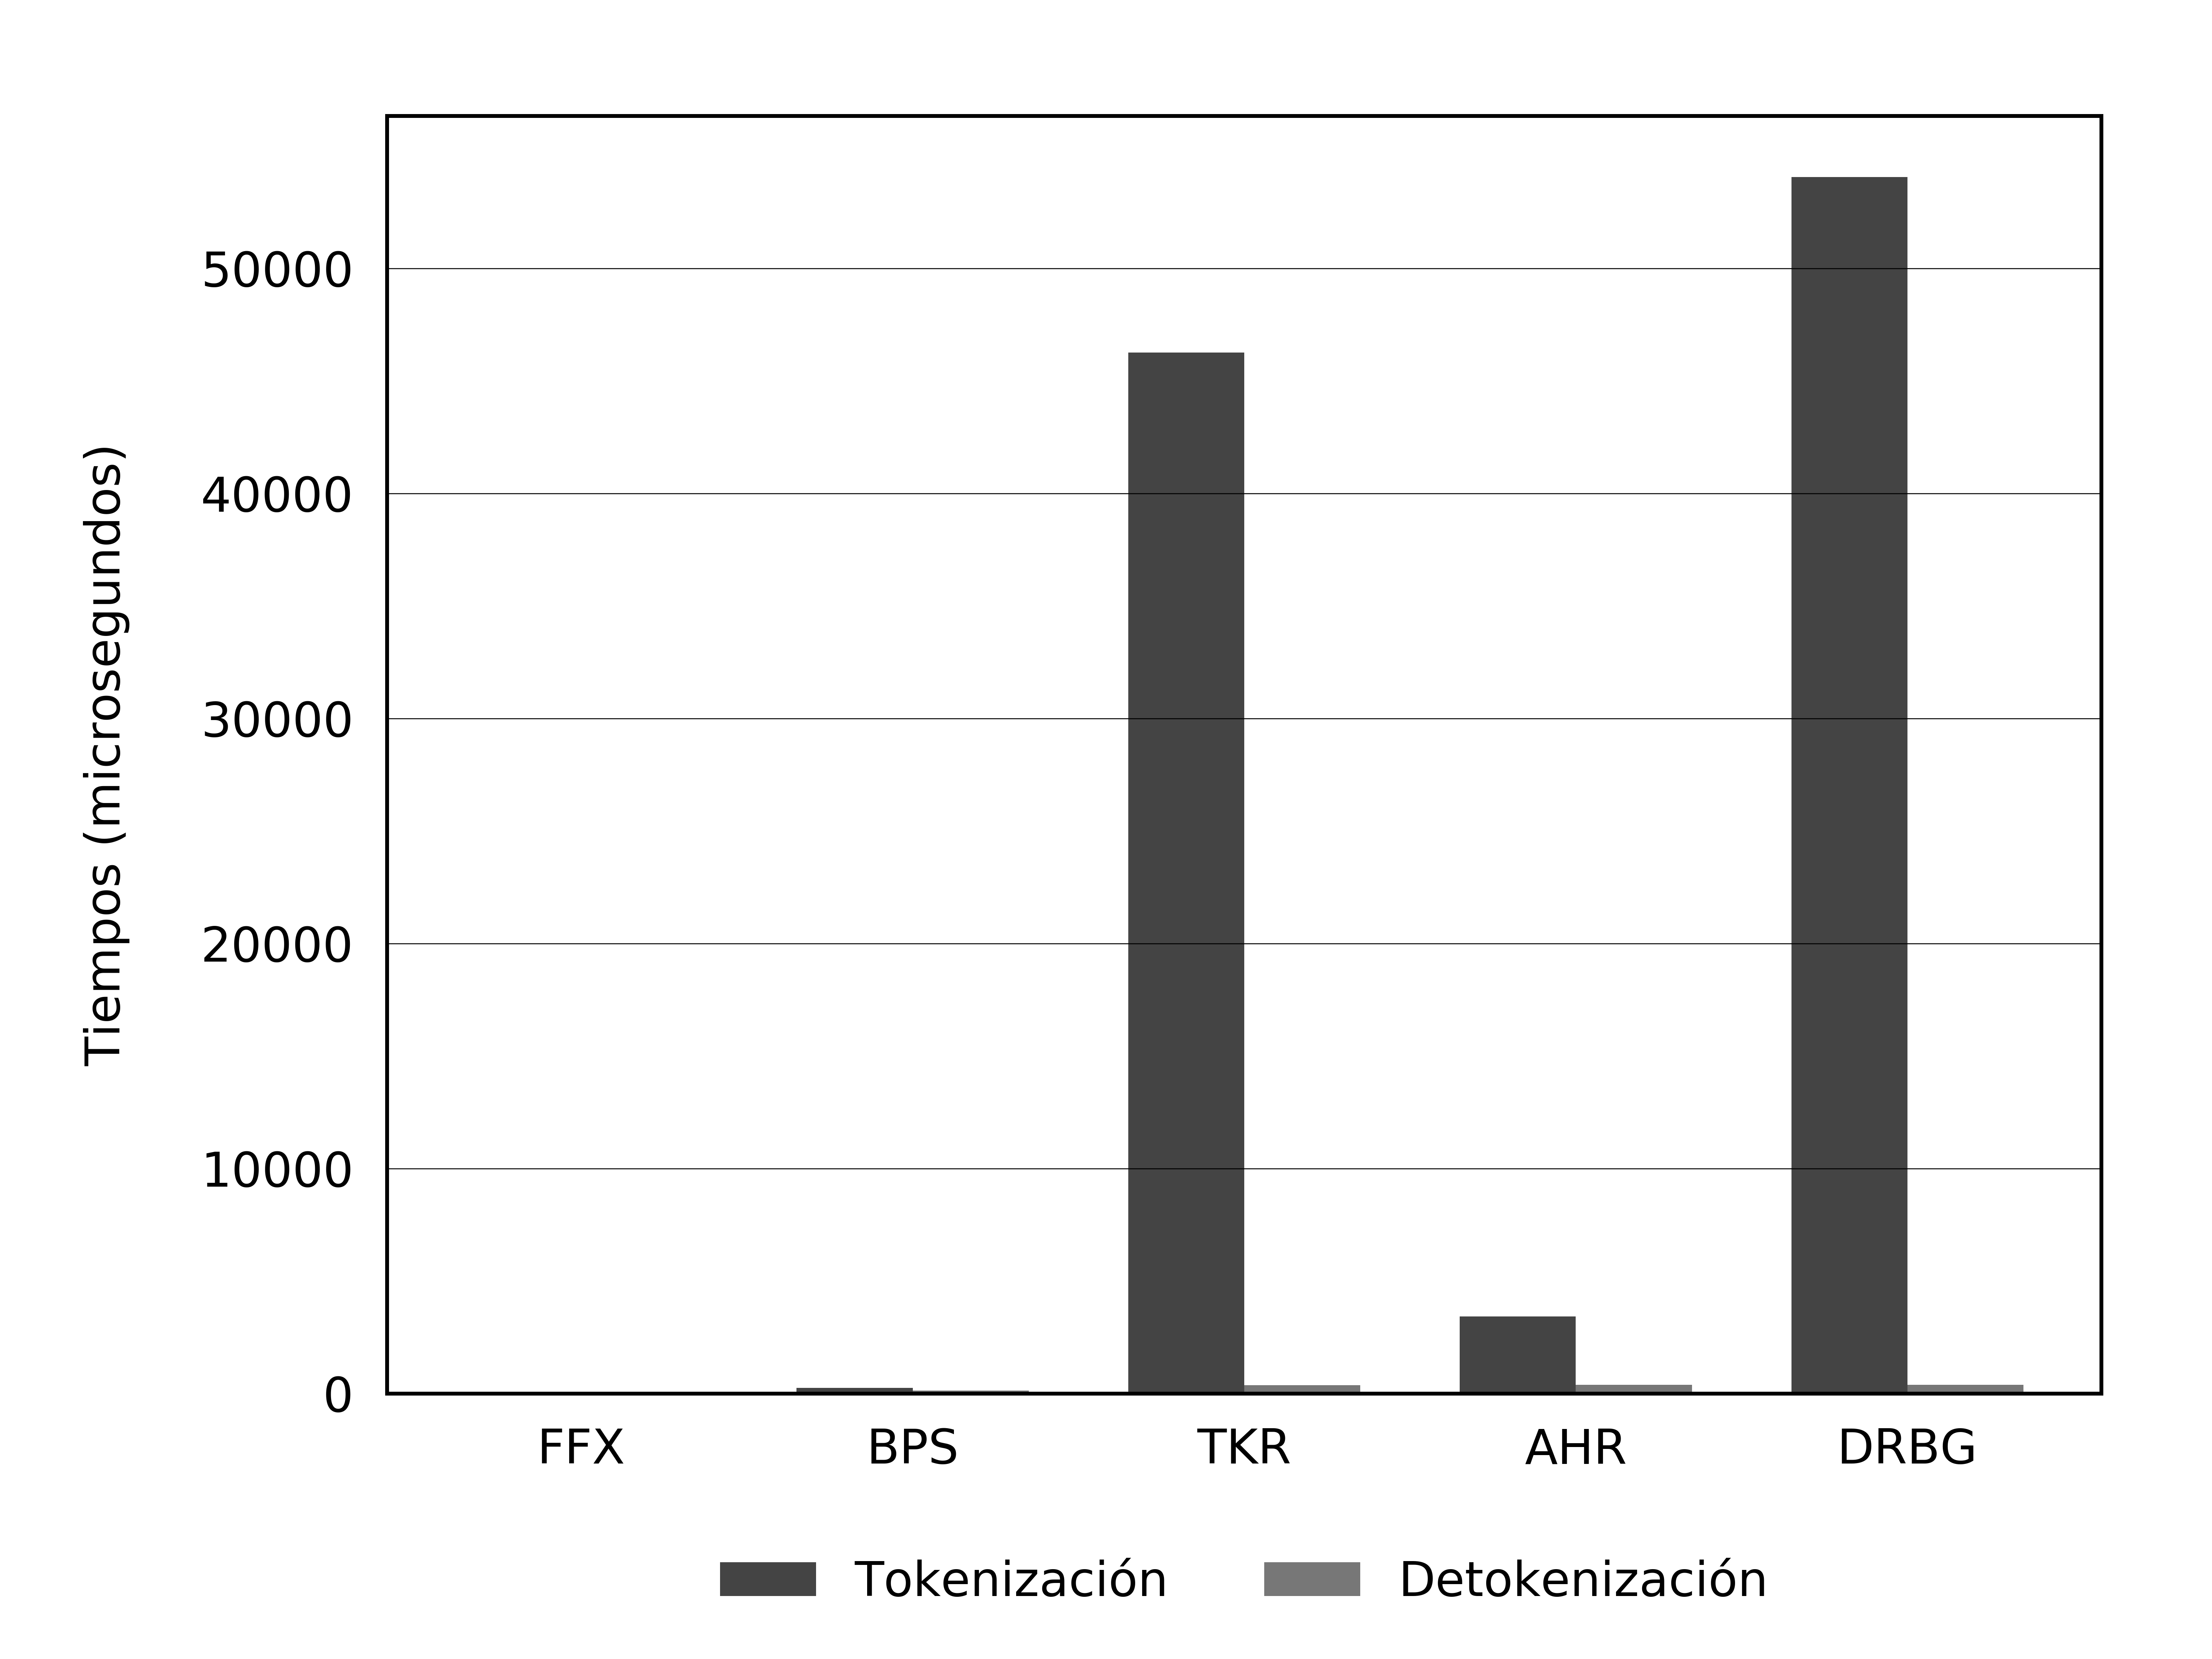
\includegraphics[width=0.9\linewidth]
      {../../articulo-rci/tiempos_unitarios.png}
      \caption{Tokenización y detokenización.}
  \end{figure}
\end{frame}

\begin{frame}{Resultados}
  \begin{figure}[H]
    \centering
    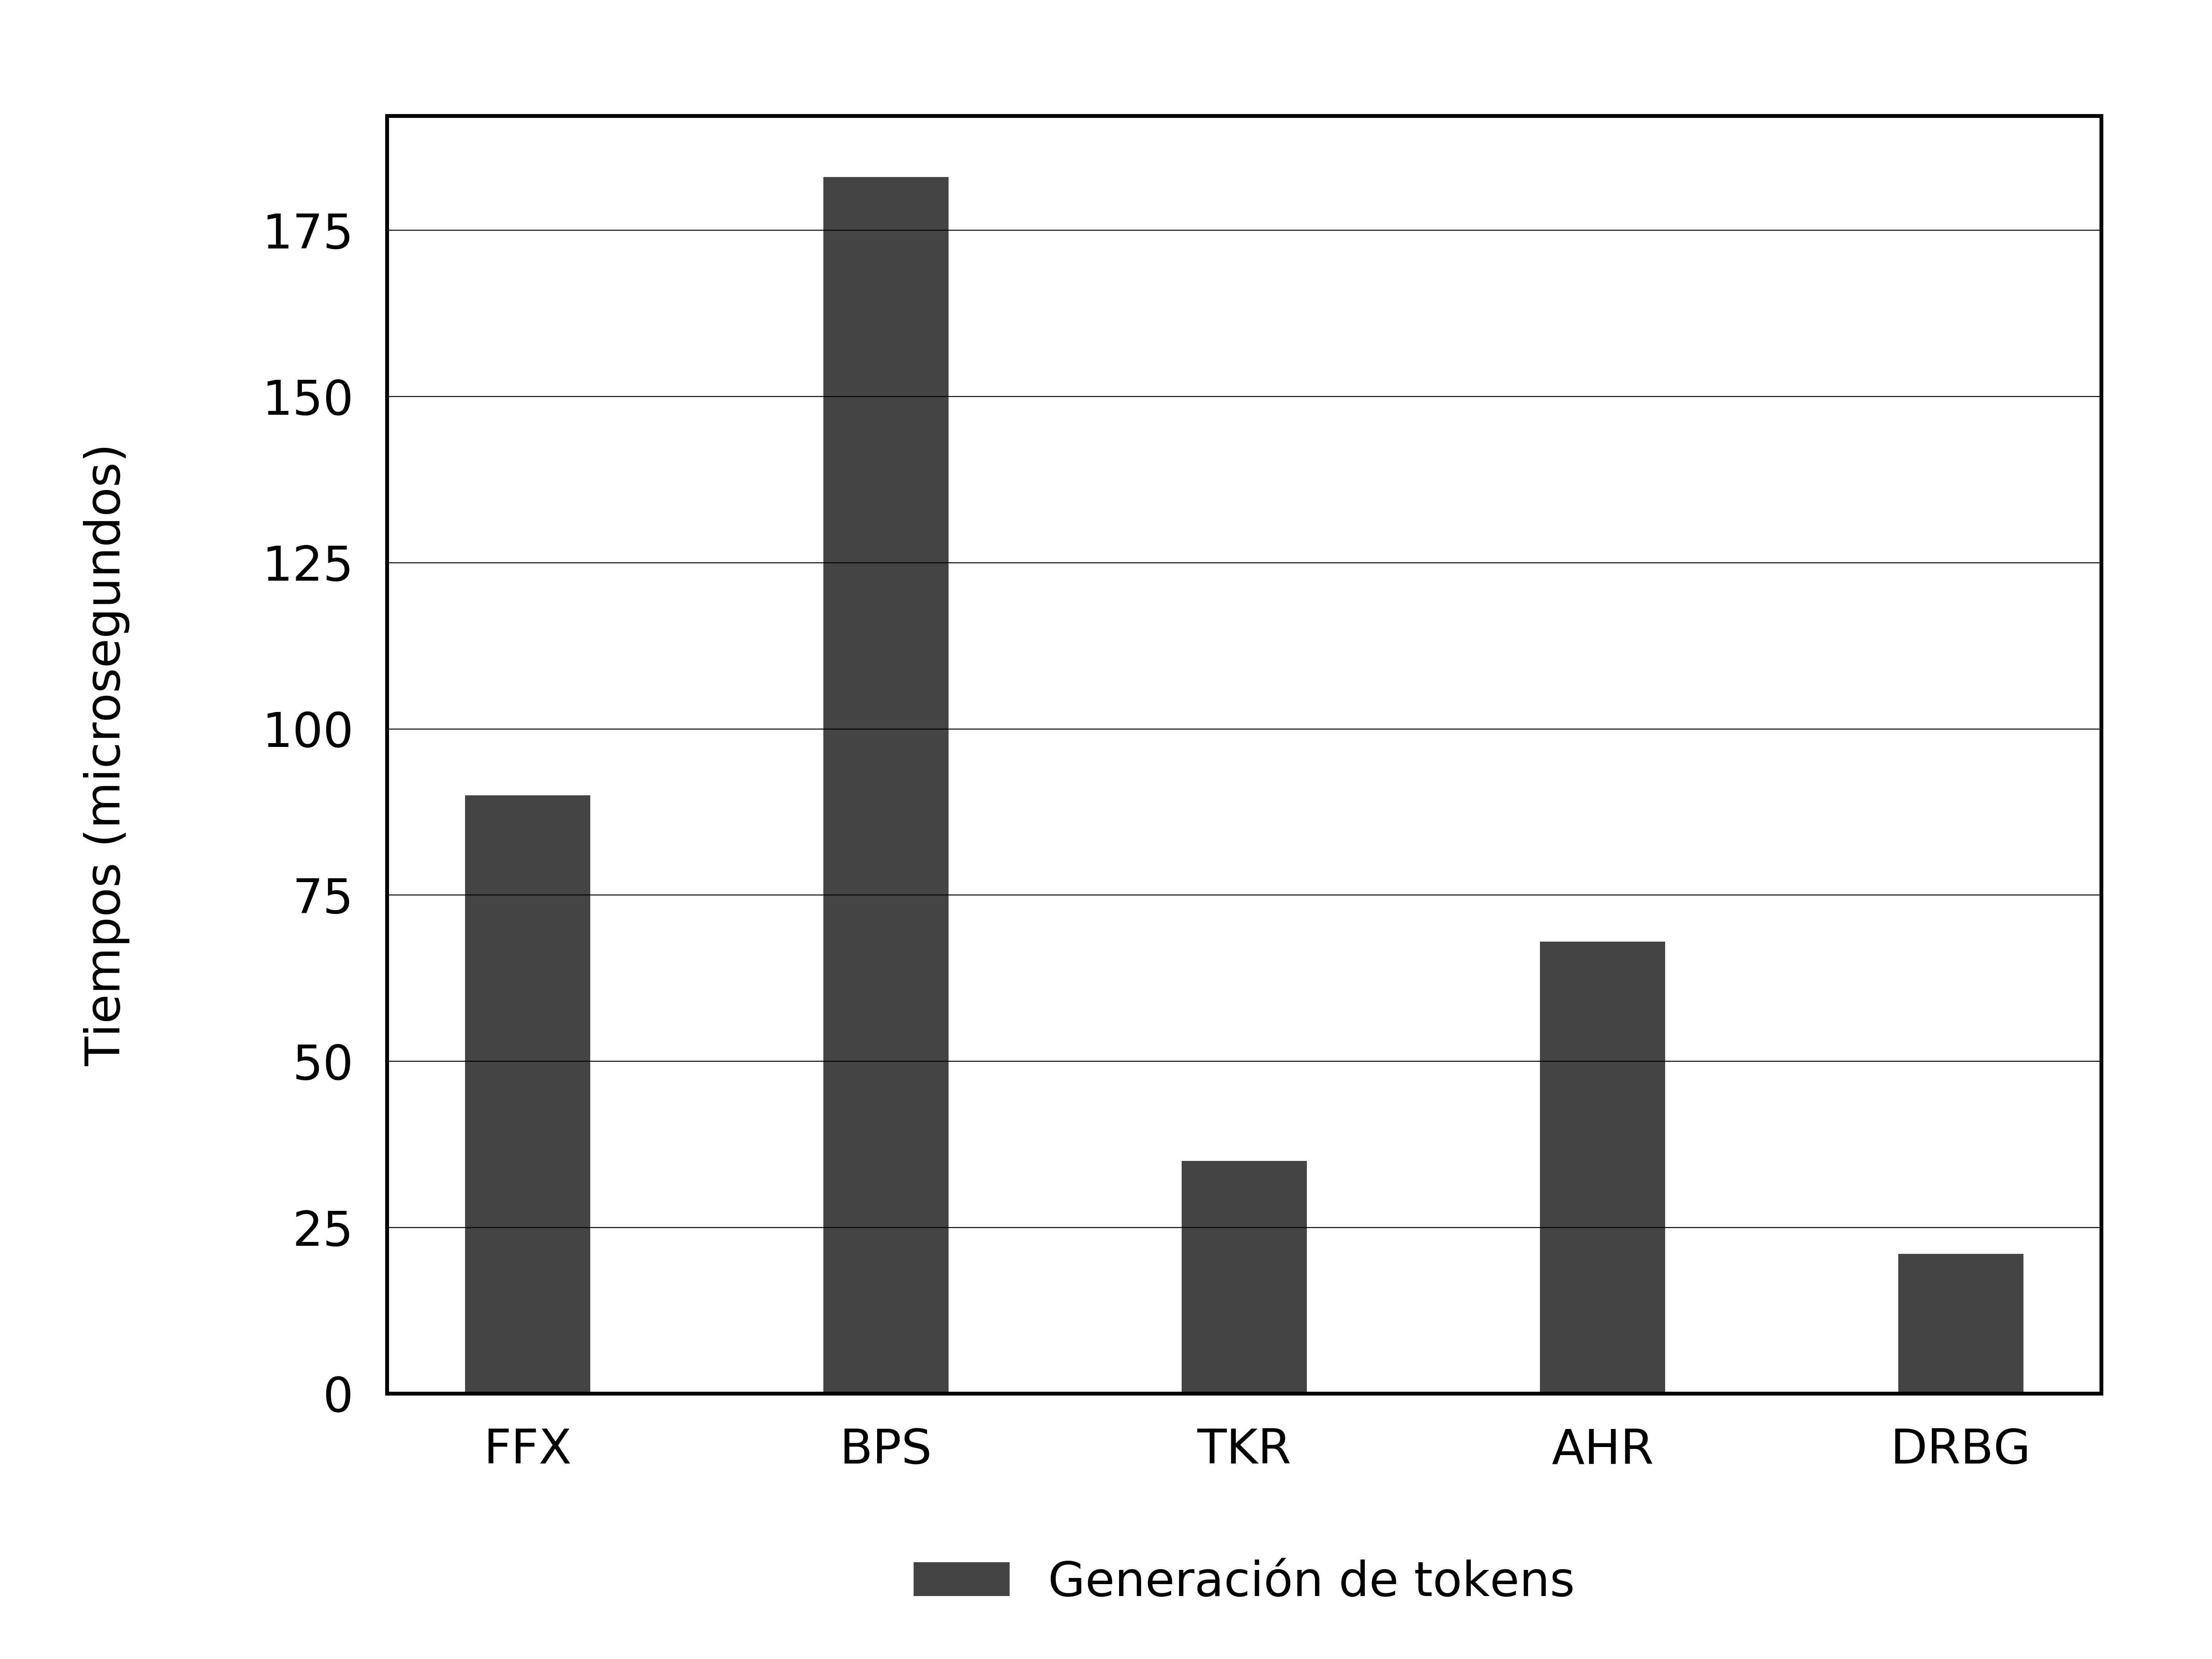
\includegraphics[width=0.9\linewidth]
      {../../articulo-rci/tiempos_tokenizacion.png}
      \caption{Generación de tokens.}
  \end{figure}
\end{frame}

\begin{frame}{Conclusiones}
  \begin{itemize}
    \item La tokenización es una aplicación de la criptografía.
    \item La denominación \textit{no criptográfica} del PCI es contradictoria.
    \item Los algoritmos reversibles son más últiles cuando se necesita tanto
      tokenizar como detokenizar con frecuencia.
    \item Los algoritmos irreversibles son más últiles cuando se requiere
      detokenizar con frecuencia.
  \end{itemize}
\end{frame}
